\section{Methodology}
\subsection{\textbf{Project Management}}
\begin{figure}
    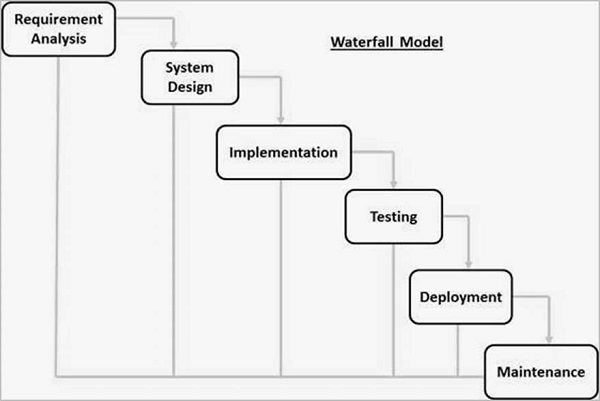
\includegraphics[width=.3\textwidth]{images/sdlc_waterfall_model.jpg}
    \caption{Flow graph showing steps of waterfall method \cite{waterfallimage}}
    \Description{Flow graph showing steps of waterfall method}
    \label{fig:waterfall}
\end{figure}
When choosing methodologies the student had 2 choices, to use a traditional software management technique such as Waterfall or a more modern approach such as Agile.
Waterfall is as described by Dr. Winston W. Royce \cite{waterfall} and as shown in Figure \RefFig{fig:waterfall}.
To be a management strategy in which the stages are quite rigid and unchanging, best suited to a project that is less likely to have changes during the development process
as the subject area being explored was new to the student, it was going to be likely to see change within requirements. The creation of
an artifact for end users and the communication with them during the process.
Whereas Waterfall is a rigid methodology thriving on predefined requirements Agile, as described in The Agile Manifesto
\cite{agile} allows for constantly changing requirements, adapting to the needs of the project and the end user and often working better
for smaller projects \cite{waterfallvsagile}.
\begin{figure}
    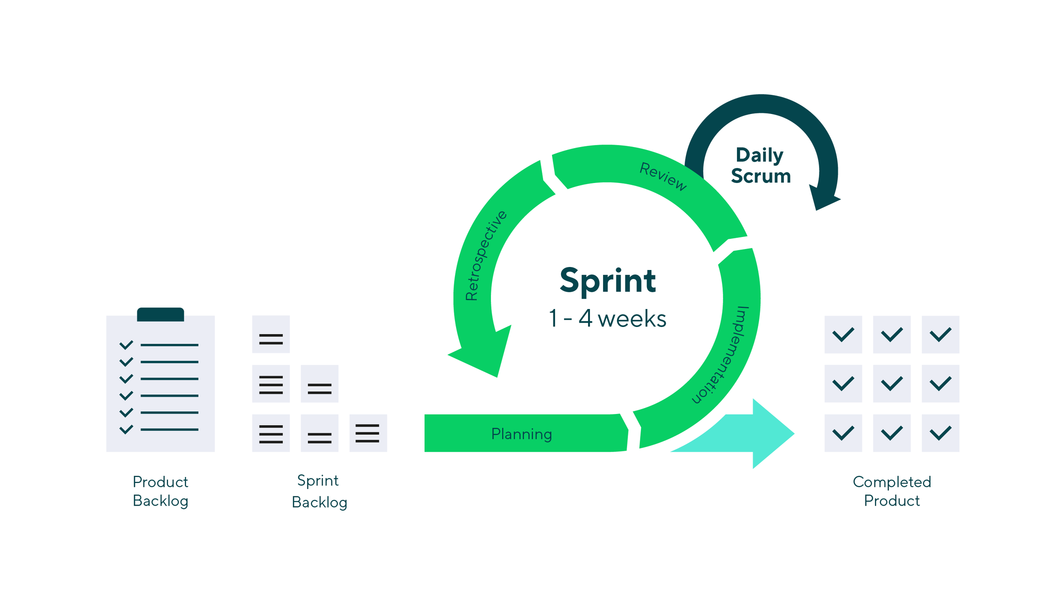
\includegraphics[width=.4\textwidth]{images/scrum-cycle-resized.png}
    \caption{Steps of a sprint \cite{sprints}}
    \Description{Steps of a sprint}
    \label{fig:sprints}
\end{figure}
With this information in mind, the student took the approach of implementing agile with 2 week long sprints \RefFig{fig:sprints}.
\begin{figure}
    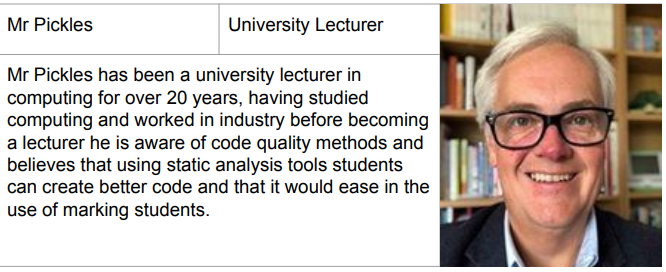
\includegraphics[width=.3\textwidth]{images/user-personas.png}
    \caption{Lecturer User Persona, see appendix D}
    \Description{Lecturer User Persona}
    \label{fig:userpersona}
\end{figure}
\subsubsection{\textbf{Creation of User Personas}}
User personas are an idea of a stereotypical user within a system. The student created 3 user stories to help better understand the end users of the system, these include
Lecturer, Developer and Student. See an example in Figure \RefFig{fig:userpersona} See Appendix D.

\subsubsection{\textbf{Creation of User Stories}}
User Stories were created with the User Personas in mind. User Stories are a clear and brief description of functionality that valuable to end users \cite{userStories}.
\begin{figure}
    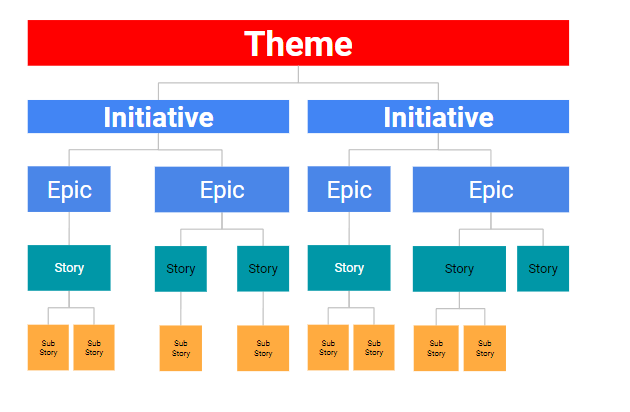
\includegraphics[width=.5\textwidth]{images/user-stories-structure.png}
    \caption{Structure of User Stories, See Appendix E}
    \Description{Structure of User Stories}
    \label{fig:userstorytheme}
\end{figure}
\begin{figure}
    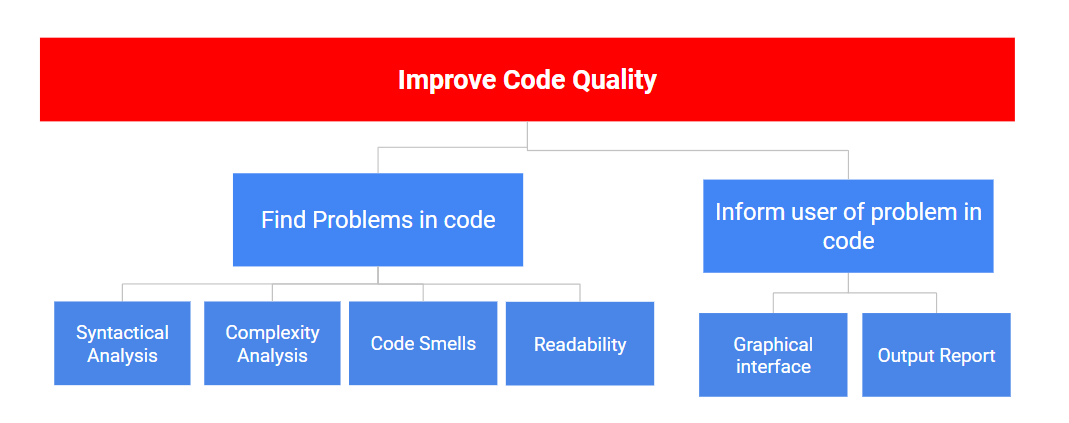
\includegraphics[width=.5\textwidth]{images/user-stories-structure-filled.png}
    \caption{User Stories Theme, Initiatives and Epics, See Appendix E}
    \Description{User Stories Theme, Initiatives and Epics, See Appendix E}
    \label{fig:userstories}
\end{figure}
Within the process of creating User Stories, a structure was created as shown in Figure \RefFig{fig:userstorytheme} and Figure \RefFig{fig:userstories}.
A theme is the Overall idea of what we are trying to create, in a larger organisation or project there could be multiple themes although as the project is limited in 
scope there is only one theme, the student felt it was prudent to ensure that the overall goal for the project to be instantiated.
An Initiative is downstream from the Theme, it is something that we want to achieve and it's Epics will again be lower level ideas of how to 
achieve this. Within an epic we finally have our user stories which describe a goal from the perspective of a user. Each User Story may have Sub Stories which take a 
more granular look at the component parts to complete that User Story , an example is Figure \RefFig{fig:complexity-userstory}
\begin{figure}
    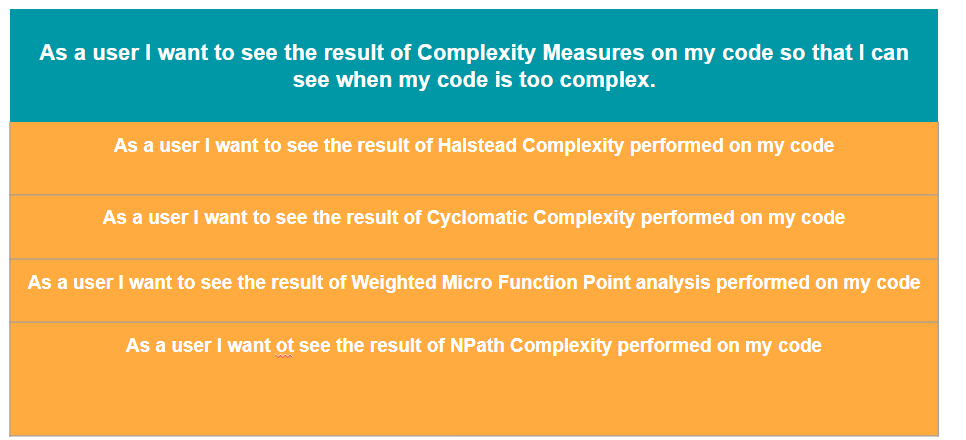
\includegraphics[width=.5\textwidth]{images/user-stories-example.png}
    \caption{Complexity Analysis User Story, See Appendix E}
    \Description{Complexity Analysis User Story, See Appendix E}
    \label{fig:complexity-userstory}
\end{figure}
\begin{figure}
    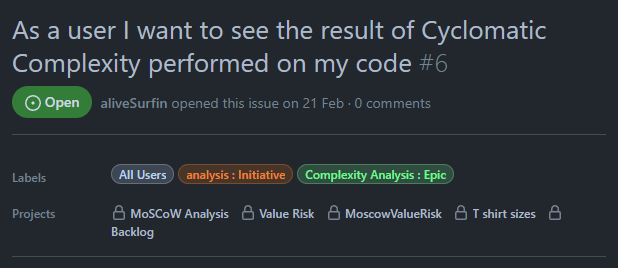
\includegraphics[width=.5\textwidth]{images/github-issue.png}
    \caption{User Story as Github Issue, See Appendix F}
    \Description{User Story as Github Issue, See Appendix F}
    \label{fig:github-issue}
\end{figure}
\subsubsection{\textbf{User Story Prioritisation and Estimation}}
User Stories were then converted to Github Issues for ease of tracking see Figure \RefFig{fig:github-issue}.
\newline
Using the Project Boards the issues were Prioritised and Estimated using a number of different methods.
The first of which is MoSCoW analysis which is a prioritisation technique in which the story is categorised into 4 distinct groups.

\begin{itemize}
    \item \textbf{MUST} - Must have this item
    \item \textbf{SHOULD} - Should complete this item if it is possible
    \item \textbf{COULD} - Could have this item if it is possible
    \item \textbf{WON'T} - Won't have this item, but would be nice to have in the future.
\end{itemize}
\cite{moscow}
User stories were separated into their distinct categories, see Appendix G.
\newline
The next method of prioritisation was Value/Risk analysis.
\begin{itemize}
    \item \textbf{Value} - How much value will completing this story item deliver to the created user personas.
    \item \textbf{Risk} - How difficult will it be to implement, will it take a long time to learn the skills associated and implement the feature. Will it have a high risk of failure?
\end{itemize}
These are then slotted into a matrix of 4 sections
\begin{itemize}
    \item \textbf{High Value - Low Risk} - These are the priority story points as they are the easiest to complete and provide the most value to users.
    \item \textbf{High Value - High Risk} - Less priority than above but still important as they provide high value to users.
    \item \textbf{Low Value - Low Risk} - Nice to have , only completed when downtime in the project.
    \item \textbf{Low Value - High Risk} - Unless there is massive downtime in development or the Risk value changes there is usually not a reason to implement this features
\end{itemize}
User Stories were separated into a Value/Risk board , see Appendix H.
\newline
These two prioritisation methods are combined to create a final priority board. This created these final sections. See appendix I.
\begin{enumerate}
    \item \textbf{High Low - Must}
    \item \textbf{High High - Must}
    \item \textbf{High Low - Should}
    \item \textbf{High High - Could}
    \item \textbf{Low Low - Could}
    \item \textbf{High High - Should}
    \item \textbf{Low High - Won't}
    \item \textbf{Low High - Could}
\end{enumerate}
These priorities would be used to determine the backlog for the project and sprints.
\newline
The final technique used was an estimation technique known as T-Shirt Sizing. Stories are estimated to be of the following sizes.
\begin{itemize}
    \item \textbf{XS}
    \item \textbf{S}
    \item \textbf{M}
    \item \textbf{L}
    \item \textbf{XL}
\end{itemize}
The first story was slotted into M and then subsequent tasks were 
added to the board in relation to the first task, this allowed the student to easier allocate based on bigger or smaller. See Appendix J.

\subsection{Test Driven Development}
For the backend coding, a Test Driven Development approach was taken, this involves writing the tests for a piece of software before you write the software 
this is said to increase code quality and also creates a cleaner design, by forcing the developer to envision the end function while writing the tests as shown in Figure 
\RefFig{fig:example-test} \cite{tdd}.
\newline
The student found this held true as although a test driven development approach was taken, a few parts of the software was written without a test in mind and these 
always turned to be less well designed and more likely to develop bugs.
\begin{figure}
    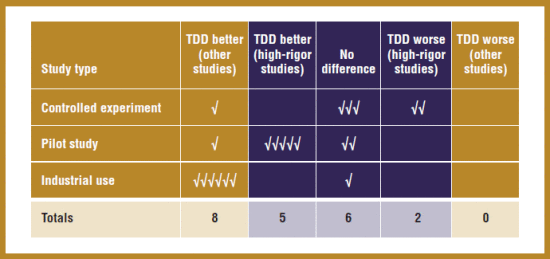
\includegraphics[width=.4\textwidth]{images/tdd effect.png}
    \caption{Effect of tdd on software outcomes \cite{tdd}}
    \Description{Effect of tdd on software outcomes}
    \label{fig:tdd}
\end{figure}
\begin{figure}[h]
\begin{lstlisting}[language=Javascript]
import Parser from "../Parser"
// table of tests [program,expectedOutput]
const testTable = [
    [``, {
        "type": "Program",
        "body": []
    }]        
]
        
const parser = new Parser()
describe('Testing empty program ', () => {
    describe.each(testTable)('parsing %s', ((program, expected) => {
        
        test(`returns ${JSON.stringify(expected)}`, () => {
            expect(parser.parse(program)).toEqual(expected)
        })
    }))
})
\end{lstlisting}
    \caption{Empty Program Parser test from "/parsing/parser/tests/empty-program.test.js" See Appendix K}
    \Description{Empty Program Parser test from "/parsing/parser/tests/empty-program.test.js" See Appendix K}
    \label{fig:example-test}
\end{figure}

\subsection{Summary}
In summary the student decided to use an agile management method, utilising stories and a backlog to ensure development. As well as using test driven development to ensure 
the quality of their software.